\subsection{Diagrama de Clases}

En el siguiente diagrama se ve reflejado que una mesa se relaciona con dos presidentes de mesa, pudiendo ser o no la misma clase. Esto se debe a que el presidente de mesa que es designado por el Ministerio posee el libre albedr\'io de no presentarse. Sin embargo, este podr\'a ir a votar y mientras no llegue primero entre los electores ser\'a considerado como un elector m\'as.\\


Por cada Presidente, existe otra entidad distinta Elector, la cual indica si dicho presidente vot\'o o no, as\'i como tambi\'en la informaci\'on pertinente de un elector.\\

Un elector puede tener una boleta en blanco, una boleta con voto grabado o ninguna bolea. En el caso de que haya impreso una boleta, se arrepienta y pida otra(s), se considerar\'a a la boleta con voto grabado como a la \'unica boleta insertada en la urna. Por lo que al modelo no le importan las boletas impresas descartadas.\\

El modelo plantea que es correcto cuando los hash de los c\'odigos coinciden, tanto con el c\'odigo original como el que est\'a en las m\'aquinas y en los pendrives. Es responsabilidad de los fiscales y presidentes corroborar y mantener que esto sea as\'i.\\


\newpage

\begin{figure}[h!]
  \begin{center}
	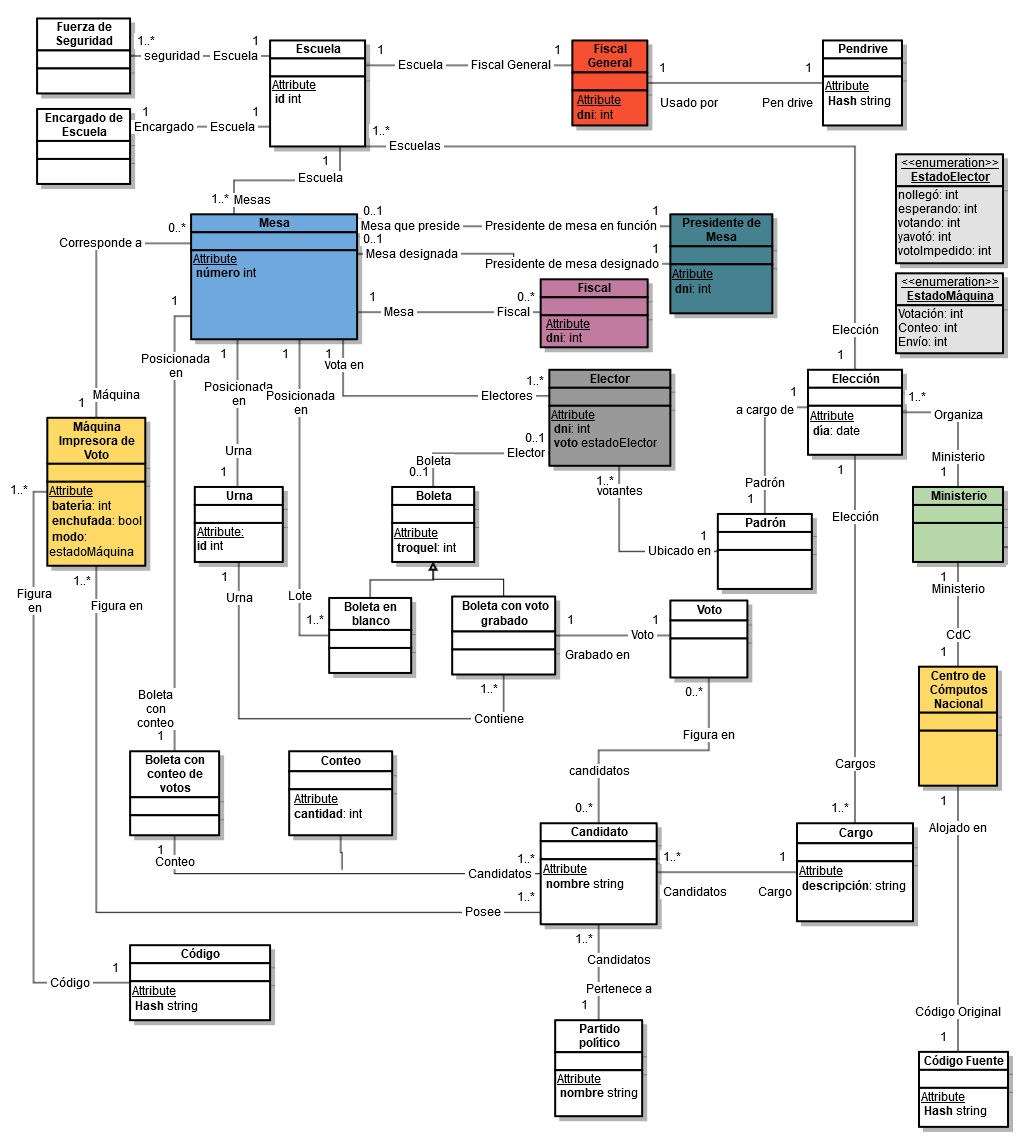
\includegraphics[scale=0.60]{imagenes/clases.png}
  \end{center}
\end{figure}

\newpage

\subsubsection{OCL}

\subsubsection*{Mesa}

\textit{context Mesa
inv}
\begin{enumerate}

\item \textbf{Los n\'umeros de las mesas son únicos.}

$Mesa.AllInstances \rightarrow forAll(m_1, m_2 | m_1.numero <> m_2.numero)$

\item  \textbf{No hay dos mesas con el mismo fiscal.}

$Mesa.AllInstances \rightarrow forAll(m_1, m_2 | m_1.Fiscal.dni <> m_2.Fiscal.dni)$

\item \textbf{No hay dos mesas con electores en común.}

$Mesa.AllInstances \rightarrow \\
 forAll(m_1, m_2 | m_1.Electores \rightarrow \\
 forAll(e_1 | m_2.Electores \rightarrow Select(e_2 | e_1.dni==e_2.dni) \rightarrow Size() == 0))$

\item \textbf{No hay dos mesas con el mismo presidente de mesa.}

$Mesa.AllInstances \rightarrow \\
forAll(m_1, m_2 | m_1.PresidenteDeMesaDesignado.dni <> m_2.PresidenteDeMesaDesignado.dni $ AND $ 
m_1.PresidenteDeMesaDesignado.dni <> m_2.PresidenteDeMesaEnFuncion.dni ) \\ $
 AND $\\
 Mesa.AllInstances \rightarrow \\
forAll(m_1, m_2 | m_1.PresidenteDeMesaEnFuncion.dni <> m_2.PresidenteDeMesaDesignado.dni $ AND $ 
m_1.PresidenteDeMesaEnFuncion.dni <> m_2.PresidenteDeMesaEnFuncion.dni ) $

\item \textbf{No puede haber un fiscal y un presidente de mesa con el mismo dni.}

$ Mesa.AllInstances \rightarrow forAll(m_1, m_2 | m_2.Fiscal \rightarrow Size() > 0 $ IMPLIES $  m2.Fiscal \rightarrow \\ 
forAll( f | m_1.PresidenteDeMesaDesignado.dni<>f.dni $ AND $ m_1.PresidenteDeMesaEnFuncion.dni<>f.dni))$

\item \textbf{Los presidentes de mesa votan en la misma mesa que son presidentes.}

$self.Electores \rightarrow Exists(e | self.PresidenteDeMesaDesignado.dni == e.dni) \\ $
 AND $ \\
 self.Electores \rightarrow Exists(e | self.PresidenteDeMesaEnFuncion.dni == e.dni) $

\item \textbf{La cantidad de Boletas Sin voto grabado y con voto grabado de la mesa debe ser mayor o igual a la cantidad de electores de dicha mesa.}

$self.Lote \rightarrow Size() + self.Urna.Contiene \rightarrow Size () \geq self.Electores \rightarrow Size()$

\item \textbf{La cantidad de Boletas Con voto grabado de la mesa debe ser menor o igual a la cantidad de electores de dicha mesa.}

$self.Urna.Contiene  \rightarrow  Size() \leq self.Electores \rightarrow Size()$

\item \textbf{No hay dos personas votando a la vez en la misma mesa.}

$self.Electores \rightarrow select( e | e.voto == votando) \rightarrow Size() \leq 1 $

\item \textbf{Si la máquina está en modo votación es porque s\'olo un elector, o ninguno, está votando (No puede haber dos electores por mesa votando a la vez).}

$self.Maquina.modo == votacion$  IMPLIES  $ \\
self.Electores \rightarrow select(e | e.voto == votando) \rightarrow Size() \leq 1 \\ $
 AND $ \\
 self.Electores \rightarrow select(e | e.voto == votando) \rightarrow Size() \leq 1 $  IMPLIES  $ \\
 self.Maquina.modo == votacion $

\item \textbf{Si la máquina está en modo conteo es porque no hay ningún elector de la mesa votando o esperando para votar.}

$self.Maquina.modo == votacion$  IMPLIES  $ \\
self.Electores \rightarrow select(e | e.voto == votando$ OR $e.voto == esperando) \rightarrow Size() = 0 \\ $
 AND $ \\
 self.Electores \rightarrow select(e | e.voto == votando$ OR $e.voto == esperando) \rightarrow Size() = 0 $  IMPLIES  $ \\
self.Maquina.modo == votacion $

\item \textbf{La máquina de la mesa puede estar en modo votación o conteo pero no en envio.}

$self.Maquina.modo <> envio$

\item \textbf{Todos los candidatos de la elecci\'on est\'an en la boleta de conteo de votos (incluyendo cuando la cantidad de votos recibida por el candidato en esa mesa fuese 0).}

$self.Escuela.Eleccion.Cargos \rightarrow \\
forAll(car | car.Candidatos \rightarrow \\
forAll(can_1 | self.BoletaConConteo.Candidatos \rightarrow \\
Exists(can_2| can_1.nombre == can_2.nombre $ AND $car.descripcion==can_2.cargo.descripcion)))$

\item \textbf{El hash del código de la M\'aquina es el mismo que el hash del código fuente del Ministerio. }

$self.Maquina.Codigo.Hash == self.Escuela.Eleccion.Ministerio.CdC.CodigoOriginal.hash$

\item \textbf{El hash del código del Ministerio es el mismo que hash de todos los pendrives de los fiscales.}

$self.Escuela.FiscalGeneral.PenDrive.Hash == self.Escuela.Eleccion.Ministerio.CdC.CodigoOriginal.hash$

\item \textbf{Si alg\'un elector vot\'o, debe haber votado el presidente mesa antes.}

$self.Electores \rightarrow \\
Exists (e | e.dni <> self.PresidenteDeMesaEnFuncion.dni $ AND $e.voto==yavoto)$ IMPLIES $\\
self.Electores \rightarrow select(v | v.dni==self.PresidenteDeMesaEnFuncion.dni) \rightarrow \\
forAll(p | p.voto==yavoto)$

\item \textbf{La elecci\'on a la que corresponde la mesa es la misma que la que le corresponde a su escuela.}

$self.Electores \rightarrow forAll (e | e.UbicadoEn.AcargoDe.dia == self.Escuela.Eleccion.dia)$

\item \textbf{Los electores est\'an en el padr\'on de la Elecci\'on que se est\'a llevando a cabo.}

$self.Electores \rightarrow forAll(e | e.UbicadoEn.AcargoDe.dia == self.Escuela.Eleccion.dia)$

\item \textbf{Los votos que figuran en las boletas de la urna son para candidatos y cargos de la elecci\'on que se est\'a llevando a cabo.}

$self.Urna.Contiene \rightarrow forAll(b | \\
b.voto.Candidatos \rightarrow forAll(can_1 | can_1.Cargo.Eleccion.dia  == self.Escuela.Eleccion.dia \\
$ AND $ \\
self.Escuela.Eleccion.cargos \rightarrow Select (car | car.descripcion == can_1.cargo.descripcion).Candidatos \rightarrow Exists(can_2 | can_1.nombre == can_2.nombre)))$
\end{enumerate}

\subsubsection*{Boleta}

\textit{context Boleta
inv}

\begin{enumerate}

\item \textbf{Los id de las boletas son únicos.}

$Boleta.AllInstances() \rightarrow forAll(b_1, b_2 | b_1.troquel <> b_2.troquel)$

\item \textbf{La boleta con voto grabado tiene elector.}

$self.IsKindOf?(BoletaConVotoGrabado)$  IMPLIES  $self.Elector \rightarrow Size() == 1 $

\item \textbf{Si un elector tiene una boleta en blanco, entonces esta boleta está en la mesa que el elector vota.}

$self.IsKindOf(BoletaEnBlanco)?$ AND $self.Elector \rightarrow Size() == 1 $ IMPLIES $\\
self.PosicionadaEn.numero == self.Elector.VotaEn.numero$

\item \textbf{Si un elector tiene una boleta con voto grabado, entonces esta boleta está en la urna que el elector vot\'o.}

$self.IsKindOf(BoletaConVotoGrabado)? $  IMPLIES  $\\
self.Urna.PosicionadaEn.numero == self.Elector.VotaEn.numero$

\end{enumerate}

\subsubsection*{Boleta con Conteo de Votos}

\textit{context Boleta con Conteo de Votos
inv}

\begin{enumerate}
\item \textbf{La boleta con Conteo de votos no tiene candidatos repetidos.}

$self.Candidatos \rightarrow forAll(c_1, c_2| c_1.nombre <> c_2.nombre)$

\end{enumerate}
\subsubsection*{Conteo}

\textit{context Conteo
inv}

\begin{enumerate}

\item \textbf{La boleta con conteo tiene la cantidad de votos que recibi\'o cada candidato en esa mesa.}

$self.Cantidad == \\
self.BoletaConConteodeVotos.mesa.boletaConVotoGrabado \rightarrow \\
select(b | b.voto.candidato  \rightarrow exist(c | c==self.candidato)) \rightarrow size() $

\end{enumerate}

\subsubsection*{Voto}

\textit{context Voto
inv}

\begin{enumerate}
\item \textbf{No tiene dos candidatos con el mismo cargo.}

$self.Candidatos  \rightarrow forAll(c_1, c_2 | c_1.cargo.descripcion <> c_2.cargo.descripcion)$

\item \textbf{No tiene dos candidatos con el mismo nombre.}

$self.Candidatos  \rightarrow forAll(c_1, c_2 | c_1.nombre <> c_2.nombre)$

\end{enumerate}

\subsubsection*{Urna}

\textit{context Urna
inv}

\begin{enumerate}

\item \textbf{En una misma urna no hay dos boletas con el mismo elector.}    

$self.Contiene \rightarrow forAll(b_1, b_2 | b_1.Elector.dni<>b_2.Elector.dni)$

\item \textbf{Los id de las urnas son únicos.}

$Urna.AllInstances() \rightarrow forAll(u_1, u_2|u_1.id<>u_2.id)$
\end{enumerate}

\subsubsection*{Escuela}

\textit{context Escuela
inv}

\begin{enumerate}
\item \textbf{Los n\'umeros de las mesas son únicos.}

$Mesa.AllInstances() \rightarrow forAll(m_1, m_2|m_1.numero<>m_2.numero)$

\end{enumerate}

\subsubsection*{M\'aquina Impresora de Voto}

\textit{context M\'aquina Impresora de Voto
inv}

\begin{enumerate}
\item \textbf{La elecci\'on que corresponde a la m\'aquina es la misma elecci\'on que le corresponde a su mesa.}

$self.Posee \rightarrow forAll(can | can.cargo.Eleccion.dia == self.Escuela.Eleccion.dia)$

\item \textbf{Los candidatos que figuran en la m\'aquina deben ser candidatos y cargos que correspondan a la misma elecci\'on de la escuela en la que est\'an ubicadas.}

$self.Posee \rightarrow forAll(can_1 | self.Escuela.Eleccion.Cargos \rightarrow \\
Exists(car | car.descripcion == can_1.cargo.descripcion $ AND $car.Candidatos \rightarrow Exists(can_2| can_1.nombre == can_2.nombre)))$

\item \textbf{La m\'aquina est\'a en la misma escuela que la escuela de su mesa.}

$self.CorrespondeA \rightarrow Size() > 0$ IMPLIES $ \\
self.CorrespondeA \rightarrow forAll(m | m.Escuela.id == self.Escuela.id)$

\item \textbf{Si la m\'aquina tiene mesa, deber\'a estar enchufada.}

$self.CorrespondeA \rightarrow Size() > 0$ IMPLIES $ self.enchufada == TRUE$

\item \textbf{Si la m\'aquina no tiene mesa y est\'a prendida, deber\'a estar en modo conteo.} 

$self.CorrespondeA \rightarrow Size() == 0 $ AND $self.enchufada==TRUE$ IMPLIES $ \\
self.modo==Conteo$

\end{enumerate}

\subsubsection*{Elector}

\textit{context Elector
inv}

\begin{enumerate}
\item \textbf{Los dni de los electores son únicos.}

$Elector.AllInstances() \rightarrow forAll(e_1, e_2 | e_1.dni <> e_2.dni)$

\item \textbf{Si el elector no llegó, está esperando o no lo dejaron votar no tiene boleta.}

$self.voto==nollego $ OR $self.voto==yavoto$ OR $self.voto==votoImpedido$ IMPLIES $\\
self.Boleta \rightarrow Size() ==0$

 AND 
 
$self.Boleta \rightarrow Size() ==0$ IMPLIES $\\
self.voto==nollego $ OR $self.voto==yavoto$ OR $self.voto==votoImpedido$

\item \textbf{Si el elector está votando, tiene una boleta en blanco.}

$self.Boleta \rightarrow Size() ==1$ IMPLIES $\\
(self.Boleta.IsKindOf?(BoletaEnBlanco)$ IMPLIES $self.voto==votando$ AND

$self.voto==votando$ IMPLIES $self.Boleta.IsKindOf?(BoletaEnBlanco))$

\item \textbf{Si el elector ya votó, tiene una boleta con voto grabado.}

$self.Boleta \rightarrow Size() ==1$ IMPLIES $\\
(self.Boleta.IsKindOf?(BoletaConVotoGrabado)$ IMPLIES $self.voto==yavoto$ AND

$self.voto==yavoto$ IMPLIES $self.Boleta.IsKindOf?(BoletaConVotoGrabado))$

\end{enumerate}

\subsubsection*{Partido Pol\'itico}

\textit{context Partido Pol\'itico
inv}

\begin{enumerate}
\item \textbf{No hay dos partidos políticos con algún candidato en común.}

$PartidoPolitico.AllInstances() \rightarrow \\
forAll(p_1, p_2 | p_1.candidatos \rightarrow \\
forAll(c_1 | p_2.candidatos \rightarrow \\
forAll(c_2 | c_1.nombre <> c_2.nombre)))$

\end{enumerate}

\subsubsection*{Centro de C\'omputos}

\textit{context Centro de C\'omputos
inv}

\begin{enumerate}
\item \textbf{Hay uno solo.}

$CentroDeComputos.AllInstances() \rightarrow size()==1$
\end{enumerate}


\subsubsection*{Ministerio}

\textit{context Ministerio
inv}

\begin{enumerate}
\item \textbf{Hay un solo ministerio.}

$Ministerio.AllInstances() \rightarrow size()==1$

\end{enumerate}

\subsubsection*{Presidente de Mesa}

\textit{context Presidente de Mesa
inv}

\begin{enumerate}


\item \textbf{No puede haber un fiscal general y un fiscal con el mismo dni.}

$Fiscal.AllInstances \rightarrow \\
 forAll(f | FiscalGeneral.AllInstances \rightarrow forAll(fg | fg.dni <f.dni>))$

\item \textbf{No puede haber un fiscal general y un presidente de mesa con el mismo dni.}

$PresidenteDeMesaDesignado.AllInstances \rightarrow \\
 forAll(pd | FiscalGeneral.AllInstances \rightarrow forAll(f_1 | f_1.dni <pd.dni>)) \\ $
 AND $\\
 PresidenteDeMesaEnFuncion.AllInstances \rightarrow \\
 forAll(pf | FiscalGeneral.AllInstances \rightarrow forAll(f_2 | f_2.dni <pf.dni>))$
 
\end{enumerate}

\subsubsection*{Candidato}

\textit{context Candidato
inv}

\begin{enumerate}
\item \textbf{Los nombres de los candidatos son únicos.}

$Candidato.AllInstances() \rightarrow forAll(c_1, c_2 | c_1.nombre <>c_2.nombre)$

\end{enumerate}


\subsubsection*{Elecci\'on}

\textit{context Elecci\'on
inv}

\begin{enumerate}
\item \textbf{Las fechas de las elecciones son \'unicas.}

$Eleccion.AllInstances() \rightarrow forAll(e_1, e_2 | e_1.dia <>e_2.dia)$

\item \textbf{Los cargos que se votan en una elecci\'on son \'unicos.}

$self.Cargos \rightarrow forAll(c_1, c_2 |c_1.descripcion <> c_2.descripcion)$

\end{enumerate}

\newpage